\documentclass{article}

\usepackage{float}
\usepackage{mathtools}
\usepackage{graphicx}
\usepackage{geometry}
\usepackage{subfig}
\usepackage[table]{xcolor}
\usepackage{bera}
\usepackage{listings}
\usepackage{verbatim} 
\usepackage{fancyvrb}
\usepackage{algorithm}
\usepackage{algorithmic}
\usepackage{hyperref}
\usepackage{tikz}
    \usetikzlibrary{positioning}
\usepackage{xepersian}



\geometry{margin=20mm}

\settextfont{B Nazanin}

\graphicspath{ {./pics/} }

\definecolor{codegreen}{rgb}{0,0.6,0}
\definecolor{codegray}{rgb}{0.5,0.5,0.5}
\definecolor{codepurple}{rgb}{0.58,0,0.82}
\definecolor{backcolour}{rgb}{0.95,0.95,0.92}


\renewcommand{\algorithmicif}{\textbf{اگر}}
\renewcommand{\algorithmicthen}{\textbf{آنگاه}}
\renewcommand{\algorithmicelse}{\textbf{وگرنه}}
\renewcommand{\algorithmicprint}{\textbf{چاپ کن}}
\renewcommand{\algorithmicendif}{\textbf{پایان شرط}}

\lstdefinestyle{mystyle}{
    backgroundcolor=\color{backcolour},   
    commentstyle=\color{codegreen},
    keywordstyle=\color{blue},
    numberstyle=\tiny\color{codegray},
    stringstyle=\color{codepurple},
    basicstyle=\ttfamily\footnotesize,
    breakatwhitespace=false,         
    breaklines=true,                 
    captionpos=b,                    
    keepspaces=true,                 
    numbers=left,                    
    numbersep=5pt,                  
    showspaces=false,                
    showstringspaces=false,
    showtabs=false,                  
    tabsize=2
}

\lstset{style=mystyle}

%\lstdefinestyle{}{
%captiondirection=RTL,language=matlab
%}

\lstdefinestyle{verilog}{
captiondirection=RTL,language=Verilog
}
%\definecolor{vgreen}{RGB}{104,180,104}
%\definecolor{vblue}{RGB}{49,49,255}
%\definecolor{vorange}{RGB}{255,143,102}
%
%\lstdefinestyle{verilog-style}
%{
%    language=Verilog,
%    basicstyle=\small\ttfamily,
%    keywordstyle=\color{vblue},
%    identifierstyle=\color{black},
%    commentstyle=\color{vgreen},
%    numbers=left,
%    numberstyle=\tiny\color{black},
%    numbersep=10pt,
%    tabsize=8,
%    moredelim=*[s][\colorIndex]{[}{]},
%    literate=*{:}{:}1
%}
%\makeatletter
%\newcommand*\@lbracket{[}
%\newcommand*\@rbracket{]}
%\newcommand*\@colon{:}
%\newcommand*\colorIndex{%
%    \edef\@temp{\the\lst@token}%
%    \ifx\@temp\@lbracket \color{black}%
%    \else\ifx\@temp\@rbracket \color{black}%
%    \else\ifx\@temp\@colon \color{black}%
%    \else \color{vorange}%
%    \fi\fi\fi
%}
%\makeatother

\def\lstlistingname{کد}
\lstset{numberstyle=\tiny\lr}

\begin{document}

\begin{titlepage}
   \begin{center}
   \Large
       \vspace*{1cm}

       \textbf{گزارش پروژه‌ی درس معماری کامپیوتر}

       \vspace{0.5cm}
      پیاده‌سازی جمع‌کننده و ضرب کننده‌ها        
      
       \vspace{1.5cm}
       {علی بهمنیار - ۹۸۲۳۰۱۸}
       \vfill
 
       \vspace{0.8cm}
     	\begin{figure}[H]%
	   	 	\centering
	    	\subfloat{{
\includegraphics[height=4cm]{logo_ee}}}
	    	\quad
	   	 	\subfloat{{
\includegraphics[height=4cm]{logo_uni}}}
		\end{figure}
            
       دانشکده‌ی مهندسی برق\\
       دانشگاه صنعتی امیرکبیر\\
       دی ماه ۱۴۰۱       
   \end{center}
\end{titlepage}

\pagebreak
\tableofcontents
\pagebreak

\section{پیاده‌سازی جمع‌کننده‌ها}
\subsection{\lr{Ripple Adder}}
این جمع کننده، ساده‌ترین نوع جمع‌کننده می‌باشد و طراحی نسبتاً ساده‌ای دارد. شمای کلی این طراحی در شکل \ref{fig:rip-car-schem} مشخص است:
\begin{figure}[H]
\centering
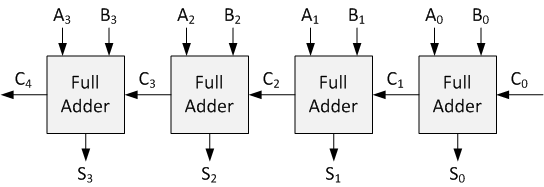
\includegraphics[width=12cm]{ripple-carry-adder-schematic}
\caption{شماتیک کلی جمع‌کننده‌ی \lr{Ripple Adder}}
\label{fig:rip-car-schem}
\end{figure}
\noindent
در این طراحی هر دو بیت توسط یک \lr{Full Adeer} با یکدیگر جمع شده، سپس بیت \lr{carry} حاصل به عنوان بیت \lr{carry} ورودی به \lr{Full Adder} بعدی داده شده تا دو بیت بعدی با یکدیگر جمع شده و این فرآیند تکرار می‌شود تا حاصل جمع نهایی ایجاد شود. \\
در این جمع‌کننده هر \lr{Full Adder} باید منتظر جواب واحد قبلی خود بماند و بنابراین برای ایجاد پاسخ نهایی سیگنال باید به ترتیب از تمامی \lr{Full Adder}ها عبور کند. به این دلیل این جمع‌کننده سرعت عملرد نسبتاً پایینی دارد.\\
پس از پیاده‌سازی این جمع‌کننده، شماتیک \lr{RTL} آن به صورت شکل \ref{fig:rip-car-rtl} می‌باشد:
\begin{figure}[H]
\centering
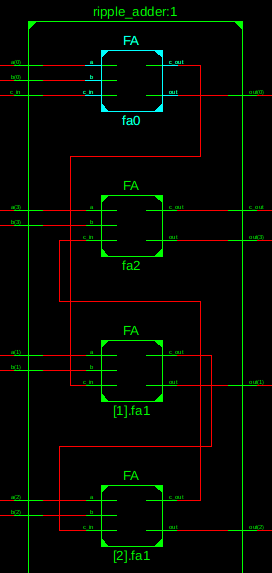
\includegraphics[height=10cm]{ripple-carry-adder-rtl}
\caption{شماتیک \lr{Ripple Adder}}
\label{fig:rip-car-rtl}
\end{figure}

\pagebreak
\subsection{\lr{Carry-Lookahead Adder}}
این جمع‌کننده نسبت به جمع‌کننده‌ی قبلی سرعت بیش‌تری دارد، اما همچنین ساختار آن نیز پیچیده‌تر است. ساختار کلی این جمع‌کننده در شکل \ref{fig:cla-schem} مشخص است:
\begin{figure}[H]
\centering
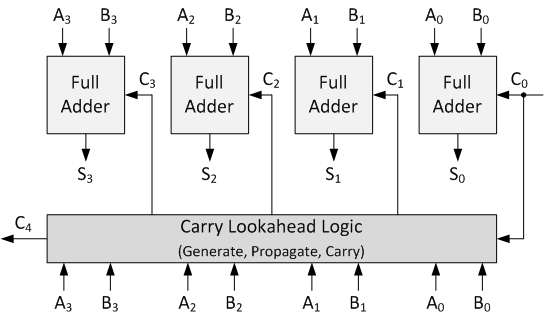
\includegraphics[width=11cm]{carry_lookahead_adder}
\caption{شماتیک کلی جمع‌کننده‌ی \lr{Carry-Lookahead}}
\label{fig:cla-schem}
\end{figure}
\noindent
در جمع‌کننده‌ی \lr{Ripple Carry} عامل اصلی تأخیر این است که هر واحد باید منتظر نتیجه‌ی بیت \lr{carry} واحد قبلی بماند، در این پیاده‌سازی برای برطرف کردن این مشکل می‌توان بیت‌های \lr{carry} را برای هر \lr{Full Adder} به صورت جداگانه توسط یک بخش مجزا محاسبه کرد. این کار باعث می‌شود تا پیچیدگی مدار بیش‌تر شود ولی سرعت انجام جمع را به طور قابل ملاحظه‌ای افزایش می‌دهد.
پس از پیاده‌سازی این جمع‌کننده، بخشی از شماتیک \lr{RTL} آن به صورت شکل \ref{fig:cla-adder-rtl} می‌باشد، از این شماتیک نیز پیچیدگی بیش‌تر مدار نسبت به راه‌حل قبلی مشخص است:
\begin{figure}[H]
\centering
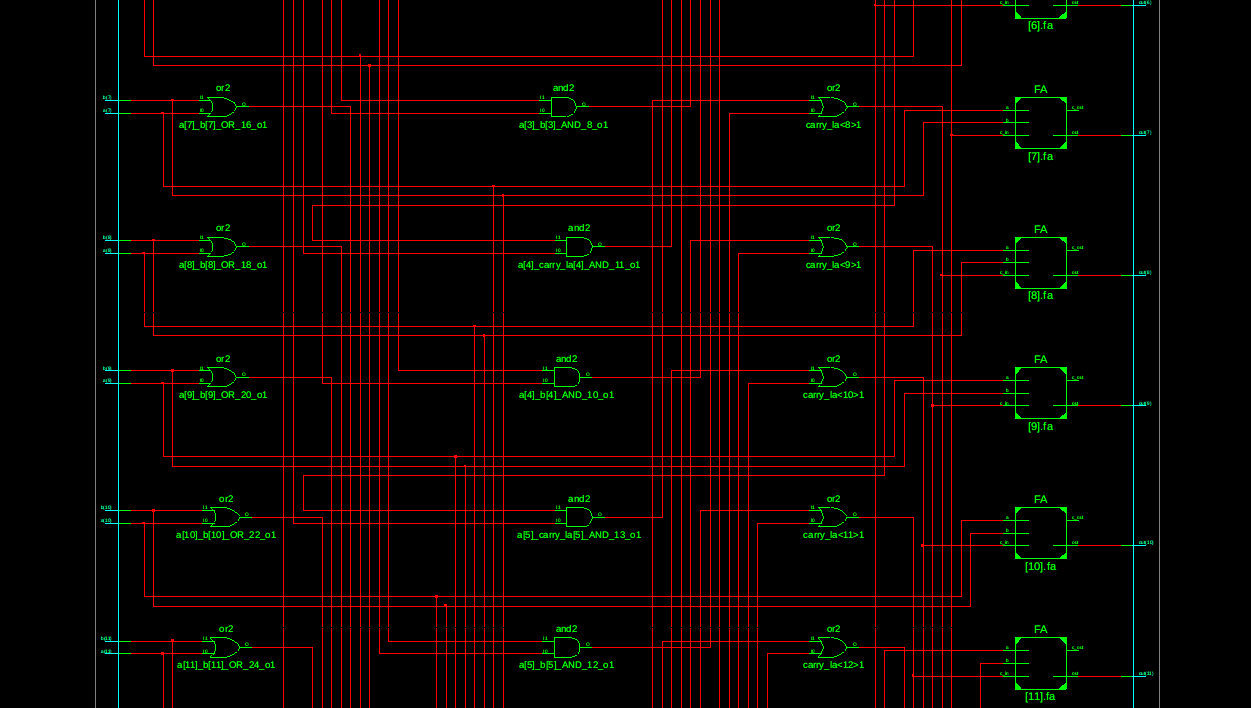
\includegraphics[width=10cm]{cla-adder-rtl}
\caption{شماتیک \lr{Carry-Lookahead Adder}}
\label{fig:cla-adder-rtl}
\end{figure}


\begin{LTR}
\begin{lstlisting}[caption={\rl{پیاده‌سازی \lr{Carry-Lookahead}}​},label=code:cla,style=verilog]
assign carry_la[j] = (a[j-1] & b[j-1]) | ((a[j-1] | b[j-1]) & carry_la[j-1]);
\end{lstlisting}
\end{LTR}
\noindent
پیاده‌سازی \lr{Carry-Lookahead} در کد \ref{code:cla} مشخص است؛ در دو صورت بیت \lr{carry} می‌بایست ۱ باشد: یا هر دو بیت ورودی ۱ باشند، یا یکی از بیت‌های ورودی به همراه بیت \lr{carry} قبلی ۱ باشند.

\subsection{\lr{Carry Select Adder}}


%\begin{latin}
%\begin{center}
%\small \begin{BVerbatim}
%NOT(0) = 1
%NOT(1) = 0
%AND(1, 1) = 1
%AND(1, 0) = 0
%AND(0, 1) = 0
%AND(0, 0) = 0
%OR(1, 1) = 1
%OR(1, 0) = 1
%OR(0, 1) = 1
%OR(0, 0) = 0
%XOR(1, 1) = 0
%XOR(1, 0) = 1
%XOR(0, 1) = 1
%XOR(0, 0) = 0
%\end{BVerbatim}
%\end{center}
%\end{latin}


%\begin{LTR}
%\lstinputlisting[caption={\rl{طراحی مدل برای دسته‌بندی دیتاست \lr{Iris}}​},label=code:iris,style=pyt]{scripts/iris.py}
%\end{LTR}

%\begin{figure}[H]
%\centering
%\includegraphics[height=9cm]{iris}
%\caption{عملکرد مدل در دسته‌بندی دیتاست \lr{Iris}}
%\label{fig:iris}
%\end{figure}
\noindent
\end{document}

